\documentclass[a4paper,titlepage]{scrartcl}
\pagestyle{plain}
\usepackage[utf8]{inputenc}
\usepackage[T1]{fontenc}
\usepackage[german]{babel}
\usepackage{float}
\usepackage{graphicx}
\usepackage{amsmath,amssymb,amstext}
\usepackage{enumerate}
\usepackage{units}

\numberwithin{equation}{section}

\title{Versuch P2-48: Ideales und reales Gas\\Vorbereitung}
\author{Gruppe Di-22\\Genti Saliu}
\date{06. Mai 2014}

\begin{document}
	\begin{titlepage}
		\maketitle
		\thispagestyle{empty}
	\end{titlepage}
	
\newpage
\pagenumbering{roman}
\tableofcontents

\newpage
\pagenumbering{arabic}

\section{Theoretische Grundlagen}

\subsection{Zustandsgrößen}
Die eindeutige Beschreibung des aktuellen Zustands eines thermodynamischen Systems erfolgt mittels der Zustandsgrößen \cite{wiki:zustandsGroesse}:
\begin{itemize}
	\item Druck $p$
	\item Temperatur $T$
	\item Volumen $V$
	\item Teilchenzahl $N$
	\item Dichte $\rho$
	\item innere Energie $U$
	\item Enthalpie $H$
	\item Entropie $S$
\end{itemize}

\subsection{Hauptsätze der Thermodynamik}
\begin{description}
\item[0. Hauptsatz] Zwei Systeme, die jeweils mit einem dritten im thermodynamischen Gleichgewicht stehen, stehen auch untereinander im Gleichgewicht. Diejenige Zustandsgröße, die bei diesen Systemen übereinstimmt, ist die Temperatur \cite{wiki:thermodynamik}.
\item[1. Hauptsatz] Die Energie eines abgeschlossenen Systems ist konstant \cite{wiki:thermodynamik}.
\item[2. Hauptsatz] Thermische Energie ist nicht in beliebigem Maße in andere Energiearten umwandelbar \cite{wiki:thermodynamik}.
\item[3. Hauptsatz] Der absolute Nullpunkt der Temperatur ist unerreichbar \cite{wiki:thermodynamik}.
\end{description}

\subsection{Ideales Gas}
Im Modell des idealen Gases werden Gasteilchen als ausdehnungslose Massenpunkte angenommen, die sich ohne Verspüren von Kräften frei durch das zur Verfügung stehenden Volumen bewegen können. Die Teilchen dürfen sich untereinander und an der Wand des Volumens stoßen. Dabei bewegen sie sich geradlinig mit konstanter Geschwindigkeit, bis ein Stoß sie in eine andere Richtung lenkt und dabei beschleunigen oder abbremsen lässt \cite{wiki:idealesGas}.\\ \\
Das ideale Gas ist eine idealisierte Modellvorstellung eines realen Gases. Damit lassen sich viele thermodynamische Prozesse von Gasen verstehen und mathematisch beschreiben. Einige Gase verhalten sich näherungsweise wie ideale Gase, z.B. Helium, Wasserstoff oder Stickstoff \cite{wiki:idealesGas}.\\ \\
Die thermische Zustandsgleichung zur Beschreibung eines idealen Gases heißt \emph{allgemeine Gasgleichung} \cite{wiki:idealesGas}:
\begin{equation*}
p \cdot V = n \cdot R \cdot T \quad
\end{equation*}
wobei $R=\unit[8.3144621]{J \cdot mol^{-1} \cdot K^{-1}}$ die universelle Gaskonstante ist. Diese Gleichung wurde aus folgenden empirischen Gesetzmäßigkeiten hergeleitet:
\begin{description}
\item[Satz von Avogadro] \emph{Gleiche Volumina idealer Gas enthalten bei gleichem Druck und gleicher Temperatur gleich viel Moleküle.} Die Anzahl der Teilchen wird in Mol gemessen, dabei gilt $\unit[1]{mol} \approx 6.022 \cdot 10^{23}$ Teilchen.
\item[Gesetz von Boyle-Mariotte] Bei konstanter Temperatur ist der Druck umgekehrt proportional zum Volumen: $p \sim V^{-1}$ $(T=const)$
\item[Gesetz von Amontons] Bei konstantem Volumen steigt der Druck wie die absolute Temperatur: $p \sim T$ $(V=const)$
\item[Gesetz von Gay-Lussac] Bei konstantem Druck steigt das Volumen wie die absolute Temperatur: $V \sim T$ $(p=const)$
\end{description}

\subsection{Reales Gas}
Beim realen Gas fallen die beim idealen Gas vorgenommenen Idealisierungen weg: die Ausdehnung der Gasteilchen wird berücksichtigt und deren Wechselwirkung geht über elastische Stöße hinaus, z.B. Van-der-Wals-Kräfte treten auf \cite{wiki:realesGas}.\\ \\
Entsprechend wird die allgemeine Gasgleichung um zwei Korrekturterme zur Van-Der-Wals-Gleichung erweitert:
\begin{equation*}
\left(p + \frac{a}{V^2}\right) \cdot \left(V - b \right)=n \cdot R \cdot T
\end{equation*}
Dabei wird die Erhöhung des Drucks im Inneren des Gases infolge der gegenseitigen Anziehung der Gasmoleküle berücksichtigt (der $\frac{a}{V^2}$-Term), sowie die Ausdehnung der Gasmoleküle mit dem Kovolumen $b$ \cite{wiki:vanDerValsGleichung}.

\section{Spannungskoeffizient $\alpha$ der Luft, absoluter Nullpunkt}
In diesem Versuch soll mit Hilfe des Jollyschen Gasthermometers der Spannungskoeffizient $\alpha$ für Luft bestimmt werden und daraus die Temperatur $\theta_0$ des absoluten Nullpunkts in Grad
Celsius berechnet werden.\\ \\
Für den Versuch wird das Jollysche Gasthermometer verwendet, welches in Abbildung \ref{fig:gasthermometer} schematisch dargestellt ist.
Das Gasthermometer besteht aus einem Glasgefäß (A), dem sogenannten Rezipienten, welches Luft enthält und sich in einem Wasserbad befindet. Über eine Kapillare (B), einen beweglichen Luftschlauch (C) und eine weitere Kapillare, die allesamt mit Quecksilber gefüllt sind, ist das Gefäß mit der Umgebung verbunden.
\begin{figure}[H]
	\centering
	\begin{tabular}{@{}r@{}}
		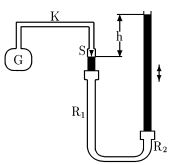
\includegraphics[width=0.4\textwidth]{bilder/gasthermometer.JPG}\\
		\footnotesize\sffamily\textbf{Quelle:} Vorbereitungshilfe \cite{vorbereitungshilfe}, Seite 1
	\end{tabular}
	\caption{Gasthermometer}
	\label{fig:gasthermometer}
\end{figure}
Für drei verschiedene Temperaturen $\theta=\unit[0]{^\circ C}$, $T_Z$, $\unit[100]{^\circ C}$, wobei $T_Z$ der Zimmertemperatur entspricht, wird die Höhendifferenz $\Delta h$ der Quecksilbersäule in den Kapillaren ermittelt. Hierzu wird die Höhe der rechten, beweglichen Kapillare jeweils so angepasst, dass der Flüssigkeitsstand
in der linken Kapillare gerade unterhalb des Dorns (D) liegt. Über den Zusammenhang
\begin{equation*}
\Delta p = \rho_{quecksilber} \cdot g \cdot \Delta h \quad \text{wobei} \quad \rho_{quecksilber} \approx \unit[13.55]{\frac{g}{cm}}
\end{equation*}
kann die Änderung des Drucks gegenüber dem Umgebungsdruck $p_b$ bestimmt werden und hieraus dann der jeweilige Druck $p$, indem der Umgebungsdruck $p_b$ hinzuaddiert wird
\begin{equation*}
p = \Delta p + p_b
\end{equation*}
weswegen noch der äußere Luftdruck $p_b$ an einem Barometer abgelesen wird.\\
Weiterhin wird das Gasvolumen V und das schädliche Volumen v abgeschätzt.\\
Zu beachten bei diesem Versuch ist, dass die Kapillare wieder gesenkt werden sollte, bevor das Gefäß abkühlen gelassen wird, da ansonsten auf Grund der Druckdifferenz Quecksilber in das Glasgefäß gelangen könnte.\\ \\
Die Bestimmmung des Spannungskoeffizienten $\alpha$ basiert auf dem Gesetz von Amontonos. Nach diesem Gesetz gilt, dass bei einer isochoren Zustandsänderung die Veränderung des Drucks $\Delta p$ eines Gases proportional zur Änderung seiner Temperatur $\Delta \theta$ ist.\\
Es gilt weiterhin folgender Zusammenhang für den Druck:
\begin{equation}
\label{eq:p}
p(T)=p_0 \cdot (1 + \alpha \cdot \Theta)
\end{equation}
wobei der Druck des Gases bei einer Temperatur $\Theta = \unit[0]{^\circ C}$ durch $p_0$ gegeben ist.
Diesen Zusammenhang macht man sich zunutze, indem man mit dem Jollyschen Gasthermometer einmal den Druck $p$ Eis für eine Temperatur $\Theta_{Eis} = \unit[0]{^\circ C}$ bestimmt, indem man den Glaskolben in Eiswasser taucht, und anschließend den Druck $p_{Sied}$ für eine Temperatur $\Theta_{Sied} = \unit[100]{^\circ C}$ misst, indem man den Glaskolben über siedendes Wasser hält.\\
Durch Umstellen der oben genannten Formel kann dann der Spannungskoeffizient $\alpha$ bestimmt werden:
\begin{eqnarray*}
p_{Sied}&=&p_{Eis} \cdot (1 + \alpha \cdot \Theta_{Sied})\\
\Leftrightarrow \alpha &=& \frac{p_{Sied}-p_{Eis}}{p_{Eis}} \cdot \frac{1}{\Theta_{Sied}}
\end{eqnarray*}
Allerdings enthält diese Gleichung die Voraussetzung, dass die Temperatur des gesamten Gasvolumens gleich ist. Dies kann aber in diesem Versuch nicht sichergestellt werden, da Teile der luftgefüllten Kapillare sich immer außerhalb des Wasserbads befinden werden. Dieses Volumen $v$ wird als schädliches Volumen bezeichnet, da es die Messung verfälscht. Es kann deswegen folgende Formel angewandt werden, um die Fehler in Folge des schädlichen Volumens $v$ zu korrigieren und um den Spannungskoeffizienten $\alpha$ zu bestimmen:
\begin{equation*}
\alpha=\frac{p_{Sied} - p_{Eis}}{p_{Eis}} \cdot \frac{1}{\Theta_{Sied}} + \frac{p_{Sied}}{p_{Eis}} \cdot \left(\gamma + \frac{1}{T_Z} \cdot \frac{v}{V}\right)
\end{equation*}
Folgende Größen wurde hierzu zusätzlich eingeführt:
\begin{itemize}
\item Wärmeausdehnungskoeffizient von Glas $\gamma$
\item Zimmertemperatur $T_Z$
\item Volumen des Gases im Wasserbad $V$
\item Schädliches Volumen v
\end{itemize}
Die Zimmertemperatur $T_Z$ lässt sich hierbei aus dem gemessenen Druck bei Zimmertemperatur $p_Z$ sowie dem Druck $p_{Eis}$ berechnen:
\begin{equation*}
T_Z=\frac{p_Z}{p_{Eis}} \cdot \unit[273.15]{K}
\end{equation*}
Aus dem idealen Gasgesetz folgt unter der Annahme, dass es eine minimale Temperatur $T_0$ gibt und dass für die gemessene Temperatur $T = T_0 + \Theta$ gilt:
\begin{eqnarray*}
p&=&\frac{k_B \cdot N \cdot T}{V}\\
\Leftrightarrow p&=&\frac{k_B \cdot N \cdot T_0}{V} + \frac{k_B \cdot N \cdot \Theta}{V}
\end{eqnarray*}
Daraus folgt:
\begin{equation}
\label{eq:nullpunktP}
p=p_0 \cdot \left(1 + \frac{\Theta}{T_0}\right)
\end{equation}
Aus den Gleichungen \ref{eq:p} und \ref{eq:nullpunktP} erhält man:
\begin{equation*}
\alpha = -\frac{1}{T_0}
\end{equation*}
Hieraus lässt sich dann auch der absolute Nullpunkt in Grad Celsius bestimmen.
\section{Bestimmung von $\frac{c_P}{c_V}$ für die Luft nach Clement-Desormes}
In diesem Versuch soll das Verhältnis der spezifischen Wärmen $\kappa = \frac{c_p}{c_v}$ mit der Methode von Clement-Desormes bestimmt werden. Dazu wird ein Gefäß mit einem angeschlossenen Manometer und einem Dreiweghahn verwendet. Je nach Hahnstellung kann durch einen Blasebalg der Druck im Gefäß erhöht werden, der Druck durch Verbindung mit der Aussenluft erniedrigt werden oder das Gefäß ver schlossen werden. Der Aufbau der Messapparat ist in Abbildung \ref{fig:clementDesormes} schematisch dargestellt.
Zur Bestimmung des Adiabatenkoeffizienten $\kappa$ wird in diesem Versuch ein Kreisprozess nahezu vollständig einmal durchlaufen, der die nachfolgend genannten Schritt umfasst und in Abbildung
\ref{fig:prozessschritte} dargestellt ist.\\
Zu bemerken bleibt, dass sich das Gefäß vor Beginn des Kreisprozesses im Gleichgewicht mit der Umgebung befindet. Die Temperatur im Gefäß entspricht hierbei der Umgebungstemperatur $T_0$, der Druck dem Umgebungsdruck $p_0$ und das Volumen dem Gefäßvolumen $V_0$.
\begin{figure}[H]
	\centering
	\begin{tabular}{@{}r@{}}
		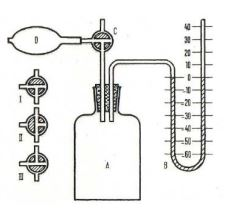
\includegraphics[width=0.4\textwidth]{bilder/clement-desormes.JPG}\\
		\footnotesize\sffamily\textbf{Quelle:} Musterprotokoll \cite{vorbereitung1}, Seite 8
	\end{tabular}
	\caption{Bestimmung von $\kappa$ nach Clément-Desormes}
	\label{fig:clementDesormes}
\end{figure}
\begin{enumerate}
\item Der Druck im Gefäß wird durch Einpumpen von Luft mittels eines Blasebalgs langsam um $\Delta p_1$ (Empfehlung nach \cite{walcher}: $\unit[100] {mm Hg}$) erhöht, wobei die Temperatur und das Volumen konstant gehalten werden.\\
Es handelt sich also um eine isochore Zustandsänderung.
\begin{eqnarray*}
V&=&V_0\\
T&=&T_0\\
p&=&p_0+\Delta p_1
\end{eqnarray*}
\item Das Gefäß wird mit der Außenluft verbunden, wodurch ein Druckausgleich stattfindet und wieder der Druck $p_0$ vorliegt. Das Volumen des Gases nimmt um $\Delta V$ zu, wobei das Gas Arbeit verrichtet, weswegen die Temperatur des Gases um $\Delta T$ abnimmt. Es handelt sich hierbei um eine adiabatische Zustandsänderung.
\begin{eqnarray*}
V&=&V_0+\Delta V\\
T&=&T_0-\Delta T\\
p&=&p_0
\end{eqnarray*}
\item  Das Gefäß wird nach erfolgtem Druckausgleich unter Zuhilfenahme des Dreiwegehahns verschlossen. Das Gasvolumen des Systems entspricht daher nun wieder dem Gefäßvolumen.\\
Es liegt eine isobare Zustandsänderung vor.
\begin{eqnarray*}
V&=&V_0\\
T&=&T_0-\Delta T\\
p&=&p_0
\end{eqnarray*}
\item  Das Gefäß erwärmt sich wieder auf Raumtemperatur, d.h. die Temperatur nimmt um $\Delta T$, wodurch der Druck im Gefäß um $\Delta p_2$ steigt. Laut \cite{walcher} liegt die Halbwertszeit für
diese Erwärmung bei ca. 10 Sekunden.\\
Es handelt sich um eine isochore Zustandsänderung.
\begin{eqnarray*}
V&=&V_0\\
T&=&T_0\\
p&=&p_0+\Delta p_1
\end{eqnarray*}
\end{enumerate}
Der Adiabatenkoeffizient $\kappa$ lässt sich (frei nach \cite{walcher}) wie folgt herleiten:\\
Die Zustände zwischen dem ersten und zweiten Prozessschritt lassen sich durch die Poissonschen Zustandsgleichungen beschreiben, wenn der adiabatische Prozess schnell genug verläuft, sodass für die Expansion des Gases nur dem Gas selbst Energie entzogen wird und sodass keine Wärmezufuhr von außen stattfindet:
\begin{eqnarray}
(p_0+\Delta p_1) \cdot V_0^{\kappa} &=& p_0 \cdot (V_0+\Delta V)^\kappa\label{eq:kappa1}\\
(T_0-\Delta T) \cdot (V_0+\Delta V)^{\kappa - 1} &=& T_0 \cdot V_0^{\kappa-1}\label{eq:kappa2}
\end{eqnarray}
\begin{figure}[H]
	\centering
	\begin{tabular}{@{}r@{}}
		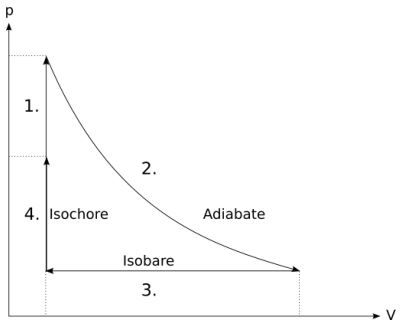
\includegraphics[width=0.6\textwidth]{bilder/prozessschritte.JPG}\\
	\end{tabular}
	\caption{Darstellung der Prozessschritte im p-V-Diagramm}
	\label{fig:prozessschritte}
\end{figure}
Die Volumenveränderung $\Delta V$ ist klein gegenüber dem Gasvolumen $V_0$, weswegen man schreiben kann:
\begin{eqnarray}
(V_0+ \Delta V)^{\kappa}&=&V_0^{\kappa} \cdot \left(1 + \frac{\Delta
 V}{V_0}\right)^{\kappa}\label{eq:kappa3}\\
 &\approx&V_0^{\kappa}+\kappa \cdot V_0^{\kappa-1} \cdot \Delta V\label{eq:kappa4}
\end{eqnarray}
Man erhält aus den Gleichungen \ref{eq:kappa1} und \ref{eq:kappa4}:
\begin{eqnarray}
\frac{\Delta p_1}{\Delta p_0}&=&\kappa \cdot \frac{\Delta V}{V_0}\label{eq:kappa5}\\
\frac{\Delta T}{T_0}&=&(\kappa - 1) \cdot \frac{\Delta V}{V_0}\label{eq:kappa6}
\end{eqnarray}
Dann folgt aus den Gleichungen \ref{eq:kappa5} und \ref{eq:kappa6}:
\begin{equation}
\label{eq:kappa7}
\frac{\Delta T}{T_0}=\frac{\kappa - 1}{\kappa} \cdot \frac{\Delta p_1}{p_0}
\end{equation}
Die Prozessschritte 3 und 4 werden durch die Zustandsgleichung idealer Gase
\begin{equation*}
\frac{p \cdot V}{T} = const.
\end{equation*}
miteinander verknüpft, sodass gilt:
\begin{eqnarray}
\frac{p_0}{p_0+\Delta p_2}&=&\frac{T_0 - \Delta T}{T_0}\label{eq:kappa8}\\
&=&1-\frac{\Delta T}{T_0}\label{eq:kappa9}
\end{eqnarray}
Setzt man Gleichung \ref{eq:kappa7} in Gleichung \ref{eq:kappa9} ein  und nutzt dabei aus, dass die Druckänderung $\Delta p_1$ deutlich kleiner als $p_0$ ist, so erhält man folgende Formel für den Adiabatenkoeffizienten $\kappa$:
\begin{equation*}
\kappa=\frac{\Delta p_1}{\Delta p_1 - \Delta p_2}
\end{equation*}
\section{Adiabatische Zustandsänderung}
In diesem Versuch soll nachgewiesen werden, dass bei der Entspannung des Gases im zweiten Prozessschritt des vorherigen Versuchs eine adiabatische Zustandsänderung angenommen werden kann.\\
Der vorherige Versuch wird zur Verifikation der adiabatischen Entspannung mehrmals durchgeführt, wobei die Zeitdauer für die Entspannung des Gases im zweiten Prozessschritt variiert wird.

\section{Bestimmung von $\frac{c_P}{c_V}$ für die Luft nach Rüchard}
In diesem Versuch soll der Adiabatenkoeffizient $\kappa$ von Luft mittels der Messmethode von Rüchard bestimmt werden.\\
Ein langes, schmales Glasrohr wird senkrecht in die Oberseite eines Gefäßes gesteckt. Anschließend wird eine kleine Stahlkugel in das Glasrohr fallen gelassen.\\
Beim Versuchsaufbau muss besondere Sorgfalt auf folgende Punkte gelegt werden:
\begin{itemize}
\item Das Glasrohr muss innen sauber sein.
\item Das Glasrohr muss absolut senkrecht stehen.
\item Das Gefäß muss bis auf das Glasrohr mit Stopfen vollständig verschlossen sein.
\item Die Kugel muss sauber sein.
\end{itemize}
Der Versuchsaufbau wird in Abbildung \ref{fig:ruechard} schematisch dargestellt.
\begin{figure}[H]
	\centering
	\begin{tabular}{@{}r@{}}
		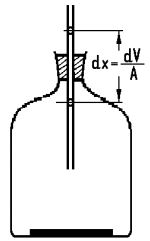
\includegraphics[width=0.25\textwidth]{Bilder/methode-ruechard.JPG}\\
		\footnotesize\sffamily\textbf{Quelle:} Vorbereitungshilfe \cite{vorbereitungshilfe}, Seite 3
	\end{tabular}
	\caption{Bestimmung von $\kappa$ nach Rüchard}
	\label{fig:ruechard}
\end{figure}
Die Kugel wird unter Zuhilfenahme eines Lederlappens (zur Schonung der Kugel) zunächst gewogen und deren Nettomasse $m$ bestimmt. Anschließend wird sie, nachdem die Dichtheit aller Stopfen am Gefäß überprüft wurde, in das Glasrohr fallen gelassen und die Schwingungszeitdauer $T$ bestimmt. Laut \cite{walcher} ist es hierbei empfehlenswert, der Bestimmung der Schwingungsdauer $T$ mindestens 5 volle Schwingungen zugrunde zu legen.\\
Nach Beendigung der Schwingung wird das Glasrohr oben mit einem Stopfen verschlossen und aus dem Gefäß entfernt, damit auf Grund des fehlenden Drucksausgleichs die Kugel beim Rausziehen des Glasrohres nicht in das Gefäß fällt. Danach lässt man die Kugel durch Entfernen des Stopfens in einen Lederlappen gleiten, um die Schwingungsdauer $T$ erneut messen zu können.\\
Weiterhin liest man an einem Barometer den Druck $p_0$ ab, um ihn anschließend korrigieren zu können.\\\\
Der Adiabatenkoeffizient $\kappa$ lässt sich (frei nach \cite{walcher}) wie folgt herleiten:
Wenn die Kugel in das Glasrohr gleitet, nimmt das Gasvolumen um $\Delta V$ ab und der Drucknimmt um $\Delta p$ ab. Die Kompression setzt sich hierbei solange fort, bis die Gegenkraft durch die Erhöhung des Drucks im Gefäß die Fallbewegung der Kugel umkehrt. Es stellt sich folglich ein Schwingungsvorgang ein, der so schnell verläuft, dass man von einer adiabatischen Zustandsänderung ausgehen kann und die folgende Poissonsche Gleichung für den Druck $p$ und das Volumen $V_0$ aufstellen kann:
\begin{equation}
\label{eq:ruechard1}
p \cdot V_0^{\kappa}=(p + \Delta p) \cdot (V_0 + \Delta V)^\kappa
\end{equation}
Unter Zuhilfenahme der Gleichung \ref{eq:kappa4} lässt sich aus der Gleichung \ref{eq:ruechard1} die Druckänderung $\Delta p$ bestimmen:
\begin{equation}
\label{eq:ruechard2}
\Delta p = - \kappa \cdot p \cdot \frac{\Delta V}{V_0}
\end{equation}
Verwendet man für die Volumenänderung $\Delta V$ die Querschnittsfläche des Glasrohres A und den Fallweg $\Delta x$ der Kugel, so ergibt sich aus Gleichung \ref{eq:ruechard2}:
\begin{equation}
\label{eq:ruechard3}
\Delta F = - \kappa \cdot \frac{p}{V_0} \cdot A^2 \cdot \Delta x
\end{equation}
Mit Hilfe der Gleichung \ref{eq:ruechard3} lässt sich dann die Bewegungsgleichung für den Schwingungsvorgang der Kugel aufstellen:
\begin{equation}
\label{eq:ruechard4}
\Delta \ddot{x} + \kappa \frac{p}{V_0} \cdot A^2 \cdot \Delta x = 0
\end{equation}
Aus der Bewegungsgleichung \ref{eq:ruechard4} lässt sich die Schwingungsdauer $T$ ableiten und nach Umformen der Adiabatenkoeffizient $\kappa$ bestimmen:
\begin{eqnarray*}
T&=&2 \pi \cdot \sqrt{\frac{m \cdot V_0}{\kappa \cdot p \cdot A^2}}\\
\Rightarrow \kappa &=& \left(\frac{2 \pi}{T}\right)^2 \cdot \frac{m \cdot V_0}{A^2 \cdot p}
\end{eqnarray*}
Zu beachten ist, dass der Druck $p$ dem Druck entspricht, wenn sich die Kugel in Ruhestellung innerhalb des Glasrohres befindet.\\
Dieser Druck setzt sich zusammen aus dem Luftdruck $p_0$ und einem Korrekturdruck $p_k$ für die Gewichtskraft der Kugel, der sich aus dem Radius $r$ und der Dichte der Kugel $\rho_{Stahl}$ berechnet.
\begin{eqnarray*}
p &=& p_0 + p_k\\
\text{mit} p_k &=& \frac{m \cdot g}{A}\\
&=& \frac{4}{3} \cdot r \cdot \rho_{Stahl} \cdot g\\
p_k &=& 1020 \cdot r
\end{eqnarray*}
\section{Dampfdruckkurve und Verdampfungswärme einer Flüssigkeit}
In diesem Versuch soll die Dampfdruckkurve von n-Hexan gemessen werden und daraus die Verdampfungswärme von n-Hexan bestimmt werden.\\ \\
Ein mit n-Hexan gefüllter Behälter wird in ein Wasserbad gebracht. Das Wasserbad wird anschließend erhitzt und danach abkühlen gelassen. Unter Verwendung eines Manometers wird der Dampfdruck $p$ und unter Zuhilfenahme eines Thermometers die Temperatur T sowohl beim Erhitzen als auch beim Abkühlen bestimmt.\\ \\
n-Heptan gehört zur Klasse von Stoffen, die – im Gegensatz zu Wasser – keine Dichteanomalie aufweisen. Das Phasendiagramm von n-Heptan entspricht daher der in Abbildung \ref{fig:phasendiagramm} gezeigten schematischen Darstellung.\\
Der Kurvenabschnitt zwischen dem Tripelpunkt und dem kritischen Punkt entspricht hierbei der Dampfdruckkurve. Bei allen Zuständen, die auf dieser Kurve liegen, befindet sich die flüssige und gasförmige Phase des n-Heptans im Gleichgewicht. Dies bedeutet, dass in diesen Zuständen genauso viel Flüssigkeit verdampft wie durch Kondensation des Dampfes entsteht. Dies ist dadurch bedingt, dass durch das Verdampfen von Flüssigkeit der Dampfdruck über der Flüssigkeit so lange zunimmt, bis er gerade dem Verdampfen entgegenwirkt.\\
Misst man den Dampfdruck über der Flüssigkeit und die Temperatur für verschiedene Gleichgewichtszustände, so kann man die Dampfdruckkurve bestimmen.
\begin{figure}[H]
	\centering
	\begin{tabular}{@{}r@{}}
		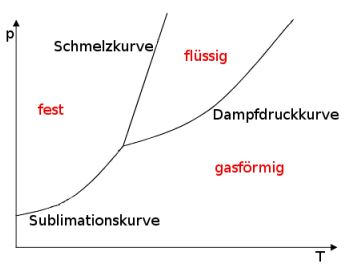
\includegraphics[width=0.6\textwidth]{bilder/phasendiagramm.JPG}\\
		\footnotesize\sffamily\textbf{Quelle:} Vorbereitungshilfe \cite{vorbereitungshilfe}, Seite 5
	\end{tabular}
	\caption{Schematische Darstellung des Phasendiagramms von n-Heptan}
	\label{fig:phasendiagramm}
\end{figure}
Aus der Dampfdruckkurve kann unter Zuhilfenahme der Clausius-Clapeyron-Gleichung
\begin{equation}
\label{eq:heptan1}
A=T \cdot (V_D-V_F) \cdot \frac{dp}{dT}
\end{equation}
die Verdampfungswärme $\Lambda$ berechnet werden, wenn das Volumen der dampfförmigen Phase $V_D$ und der flüssigen Phase $V_F$ bekannt ist.\\
Da das Volumen der flüssigen Phase $V_F$ gegenüber dem Volumen des Dampfes $V_D$ vernachlässigt werden kann, kann das Volumen $V_D$ durch das ideale Gasgesetz ausgedrückt werden, wobei es sich bei um n-Hexan um ein einmolares Gas handelt:
\begin{eqnarray}
V_D&=&\frac{n \cdot R \cdot T}{p}\label{eq:heptan2}\\
&=&\frac{R \cdot T}{p} \quad \text{mit} \quad n = 1 \label{eq:heptan3}
\end{eqnarray}
Setzt man Gleichung \ref{eq:heptan3} in Gleichung \ref{eq:heptan1} ein, erhält man:
\begin{equation*}
\Lambda = \frac{R \cdot T^2}{p} \cdot \frac{dp}{dT}
\end{equation*}
Eine nachfolgende Separation der Variablen und unbestimmte Integration der Gleichung führt zu:
\begin{equation*}
\frac{\Lambda}{T}=-R \cdot \ln(p) + const. \quad \text{mit} \quad R=\unit[8.314472]{\frac{J}{mol \cdot K}}
\end{equation*}
Durch Zuhilfenahme der linearen Regression lässt sich nun aus dieser Beziehung die Verdämpfungswärme $\Lambda$ von n-Heptan bestimmen.
Die Verdampfungswärme von n-Heptan beträgt $\Lambda = \unit[28.85]{\frac{kJ}{mol}}$.
\newpage
\bibliographystyle{plain}
\bibliography{quellen}

\end{document}